%%%%%%%%%%%%%%%%%%%%%%%%%
%% 02-STATE OF THE ART %%
%%%%%%%%%%%%%%%%%%%%%%%%%
\clearpage\section{State of the art}
This chapter will provide a general overview, in the context of Linux, of the different technologies used by the operating system to provide the foundation of "containers".

It will also expose a brief comparison between some systems which use containerization and explain which one suits ore needs better.

And finally it will present the set of tools in which our framework resides on.

\subsection{Container technology}
\paragraph{Containers.} Operating system main abstractions are processes. Processes act as instances of programs and are executed whenever the CPU schedules them. Depending on their properties they have the ability to execute diferent actions (read from file, send a packet, open a socket ...).

Containers are no different than this. They are mainly an abstraction for a process with a set properties provided the operating system by different technologies, and a supporting runtime. The main technologies are \textbf{namespaces} and \textbf{cgroups}.

And as the functionalities offered are implemented inside the kernel, they don't need to run any kind of hypervisor or virtualization. The following image illustrates this fact:

\begin{figure}[H]
	\label{fig:Virtualization vs Containers}
	\centering
	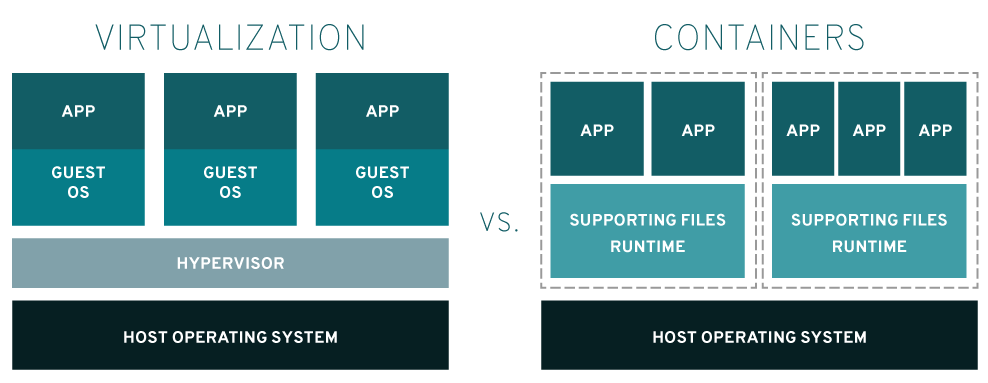
\includegraphics[width=\textwidth]{img/02/02-state-virtualization-vs-containers.png}
	\caption[Virtualization vs Containers]{\footnotesize{TODO: PONER EL LINK}}
	\TODO{poner el link}
\end{figure}

This creates a lightweight solution for applications where only one service will be running (such as a web server) without the need of setting up a whole VM with a separated kernel.

For enabling the existence of containers, the kernel offers some technologies for "isolate" containers and control their resources.

\paragraph{Namespaces.} The first kernel feature provided by the kernel, which is the main foundation for the concept of containers, are the kernel namespaces.
They are mainly and abstraction that enables the kernel to limit the context and visibility of the kernel objects. The kernel just label their resources and when it receives a request for viewing some of his objects, it only offers the ones according to the label.

In this way, different process with different labels can have separate views of the kernel objects and they are not able to access the objects different from their label.

The kernel provides 7 namespaces:
\begin{itemize}
	\item{Mount (mnt)}
	\item{Process ID (pid) (mnt)}
	\item{Network (net)}
	\item{Interprocess Communication (ipc)}
	\item{Control group (cgroup)}
	\item{UTS}
	\item{User ID (user)}
\end{itemize}

And they are manipulated using 3 syscalls:
\begin{itemize}
	\item{clone(): used with namespaces, creates a new process in the specified namespace}
	\item{unshare(): modify the context of a process}
	\item{setns(): allows attaching a process to an existing namespace}
\end{itemize}

\paragraph{Cgroups.} Control groups ("cgroups") are a kernel feature that allows the kernel to allocate resources (CPU time, system memory) to a group of process. They are not dependant of namespaces, but they are used with namespaces to limit, control and isolate resource usage.

We won't go into detail about the technologies mentioned before, but it is good to have to a general overview of the mechanisms used by the kernel.

\TODO{poner los links de las diferentes cosas}

\bigskip
\subsection{Containerization systems}
The concept of "container" is enabled by the different kernel technologies mentioned before, but there is another key element that takes part - the runtime.

The uses and systems in which containers are used nowadays vary a lot, but the key that they have in common is that they want to run some kind of application with all their dependencies in a confined environment (a.k.a the containers).

Different runtimes and systems have emerged over the recent years:
\begin{figure}[H]
	\label{fig:Runtimes containers landscape}
	\centering
	\includegraphics[width=\textwidth]{img/02/02-runtimes.png}
	\caption[Runtimes lansdcape]{\footnotesize{TODO: poner el link}}
	\TODO{poner el link}
\end{figure}

Where this thesis has been built with `lxc/lxd`, as it is intended to provide a kind of full virtual machines "container" that behaves like a normal linux distribution, whereas other systems (such as Docker) are more intended to running applications (ex: running a database service).
\TODO{
	poner aqui una comparación de los sistemas más exhaustiva??.., no lo se
	- link: https://github.com/saschagrunert/demystifying-containers
}

\subsection{LXC}
As we have stated before, the framework developed in this thesis has been constructed in top of `LXC/LXD`, which are both open source tools provided by the Linux Containers project.
\TODO{Tengo que poner aqui algun tipo de link o abreviation??}

In reality, LXD is built on top of LXC, so we will explain the two tools separated to have a general idea how their work.
\TODO{LXC/LXD as tools, projects or interfaces ??, runtimes??}

\paragraph{LXC.} LXC is a userspace interface for the kernel containment features, according to [link]. It provides a powerful API and simple tools to manage system or applications containers.

It combines namespaces and cgroups, along as other security mechanisms to provide isolated environments and contain processes.

It is formed basically by:
\begin{itemize}
	\item{C library (liblxc)}
	\item{Several languages bindings}
	\item{Set of tools for controlling containers}
	\item{Distribution templates}
\end{itemize}

Some commands for managing containers:
\begin{itemize}
	\item{Creating a container with an Ubuntu template}:
	      \begin{minted}[bgcolor=background]{bash}
host# lxc-create -n mycontainer -t ubuntu
	\end{minted}
	\item{Run a command inside the container}
	      \begin{minted}[bgcolor=background]{bash}
host# lxc-attach -n webserver -- ifconfig eth1 192.168.1.2/24
	\end{minted}
\end{itemize}

Where we can customize the containers in different ways such as:
\begin{itemize}
	\item{Attaching devices}
	\item{Configure bridges, hardware addresses, network configurations ...}
	\item{Migrate containers from one host to other host}
	\item{Set up unprivileged containers}
\end{itemize}

\subsection{LXD}
\paragraph{LXD.} LXD is a tool written in Go, defined as a system container manager which offers a user experience similar to virtual machines but using Linux contianers insted, according to [link].

Is composed basically by:
\begin{itemize}
	\item{A REST API over a local unix socket as well as over the network}
	\item{A client, provided by a new command line tool, which talks with the REST API}
\end{itemize}
so we are able to manage the containers by a REST API in a flexible and composable way.

It has also different integrations with container services along other advanced features.

It is not a rewrite of the previous tool (LXC) but a tool builded on top of it through liblxc and the Go bindings.

Some examples for interacting with containers:

\begin{itemize}
	\item{Creating a container with an Ubuntu template}:
	      \begin{minted}[bgcolor=background, breaklines]{bash}
host# lxc launch ubuntu:20.04 test
	\end{minted}
	\item{Obtain a shell inside the container named test}
	      \begin{minted}[bgcolor=background, breaklines]{bash}
host# lxc exec test bash 
	\end{minted}
	\item{Create a proxy device connecting container port 80 with host port 80}
	      \begin{minted}[bgcolor=background, breaklines]{bash}
host# lxc config device add test testport80 listen=tcp:0.0.0.0:80 connect=tcp:127.0.0.1:80 
	\end{minted}
	\item{Shared a host folder with the container test}
	      \begin{minted}[bgcolor=background, breaklines]{bash}
host# lxc config device add test devicewww disk source=/wwwdata path=/var/www/html 
	\end{minted}
\end{itemize}



\TODO{Add link for the LXD descriptions}




